\documentclass{beamer}
\usetheme{Boadilla}
%\usetheme{Frankfurt}

\usepackage{listings}
\usepackage{graphicx}
\usepackage{listings}
\usepackage{geometry} 

\usepackage{color}

\definecolor{codegreen}{rgb}{0,0.6,0}
\definecolor{codegray}{rgb}{0.9,0.9,0.9}
\definecolor{codepurple}{rgb}{0.58,0,0.82}
\definecolor{backcolour}{rgb}{0.95,0.95,0.95}
\definecolor{codered}{rgb}{1,0,0}
\definecolor{black}{rgb}{0,0,0}
\definecolor{backgroundblack}{rgb}{0.3,0.3,0.3}
\definecolor{white}{rgb}{1,1,1}

\newcommand{\listingsfont}{\fontsize{9}{9}\ttfamily}

\lstdefinestyle{mystyle}{
	backgroundcolor=\color{backcolour},   
	commentstyle=\color{codegreen},
	keywordstyle=\bfseries\color{blue},
	numberstyle=\tiny\color{codered},
	stringstyle=\color{red},
	%basicstyle=\linespread{0.8}\listingsfont,
	basicstyle=\listingsfont,
	breakatwhitespace=false,         
	breaklines=true,                 
	captionpos=b,                    
	keepspaces=true,                                    
	numbersep=5pt,                  
	showspaces=false,                
	showstringspaces=false,
	showtabs=false,                  
	tabsize=2,
	language = python,
}

\lstset{style=mystyle}

%Impostare i sottotitoli più grandi su tutte le slides
\setbeamerfont{framesubtitle}{size=\large}

\title{CNN for Cifar-10 e Cifar-100 Classification on \textit{Coral Edge TPU USB Accelerator} and \textit{ST Cloud JAM}}
\author
{}
\date{March 2020}



\begin{document}
\maketitle

\begin{frame}
\frametitle{CNN for Cifar-10 classification on computer}
\framesubtitle{Neural Network architecture}
\begin{figure}
	\centering
	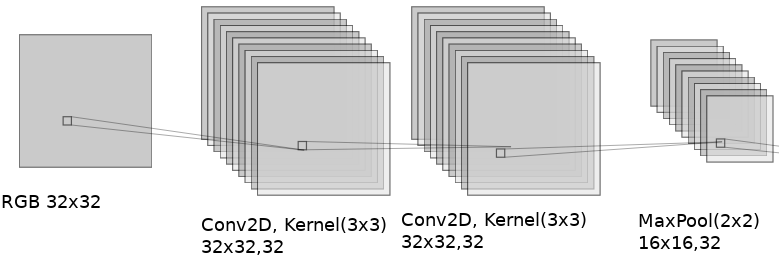
\includegraphics[scale=0.4]{pictures/cnn1_crop_labels}
\end{figure}
\end{frame}

\begin{frame}
\frametitle{CNN for Cifar-10 classification on computer}
\framesubtitle{Neural Network architecture}
\begin{figure}
	\centering
	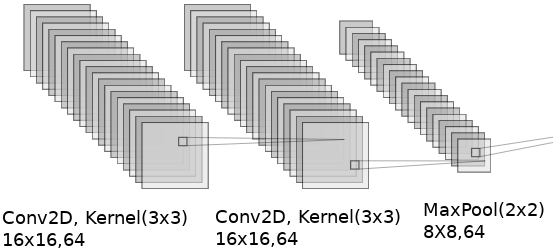
\includegraphics[scale=0.4]{pictures/cnn2_crop_labels}
\end{figure}
\end{frame}

\begin{frame}
\frametitle{CNN for Cifar-10 classification on computer}
\framesubtitle{Neural Network architecture}
\begin{figure}
	\centering
	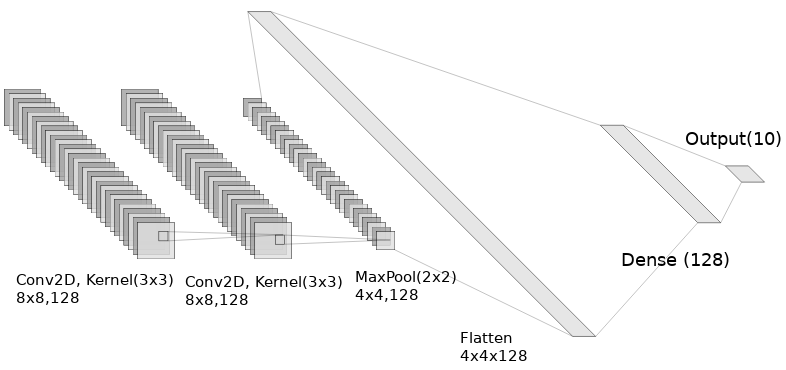
\includegraphics[scale=0.4]{pictures/cnn3_crop_labels}
\end{figure}
\end{frame}

\begin{frame}[fragile]
\frametitle{Cifar-10 random images}
\framesubtitle{Stampa di pictures random}
\begin{figure}
	\centering
	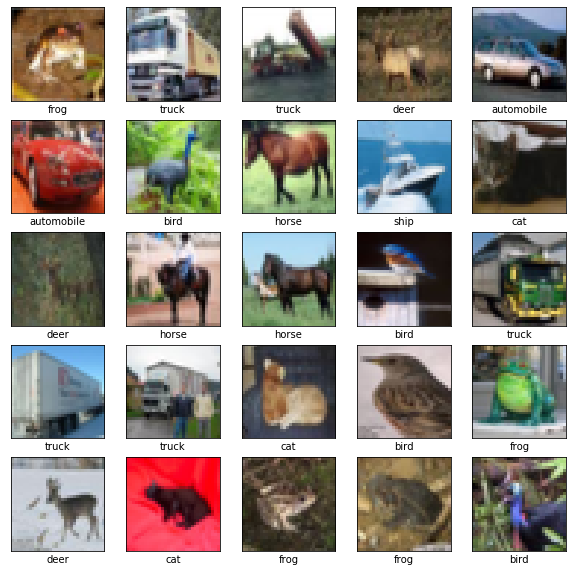
\includegraphics[scale=0.35]{pictures/index}
\end{figure}
\end{frame}

\begin{frame}[fragile]
\frametitle{CNN for Cifar-10 classification on computer}
\framesubtitle{Data Agumentation}
\begin{lstlisting}
datagen = ImageDataGenerator(
	rotation_range=15,
	width_shift_range=.1,
	height_shift_range=.1,
	horizontal_flip=True,
	zoom_range=0.5)
\end{lstlisting}
\end{frame}

\begin{frame}[fragile]
\frametitle{CNN for Cifar-10 classification on computer}
\framesubtitle{Training hyperparameters}
	\begin{lstlisting}
model.compile(loss=keras.losses.categorical_crossentropy,optimizer=keras.optimizers.Adam(),metrics=['accuracy'])
	\end{lstlisting}
\end{frame}

\begin{frame}[fragile]
\frametitle{CNN for Cifar-10 classification on computer}
\framesubtitle{Accuracy}
	\centering
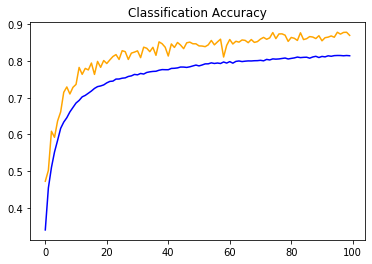
\includegraphics[scale=0.5]{pictures/Accuracy_plot_Cifar10_Keras}
\begin{lstlisting}
Epoch 100/100
782/782 [==============================] - 31s 40ms/step - loss: 0.5471 - acc: 0.8146 - val_loss: 0.3975 - val_acc: 0.8701
\end{lstlisting}
\end{frame}

\begin{frame}[fragile]
\frametitle{CNN for Cifar-10 classification on ST Cloud JAM}
\framesubtitle{Neural Network architecture}
\begin{figure}
	\centering
	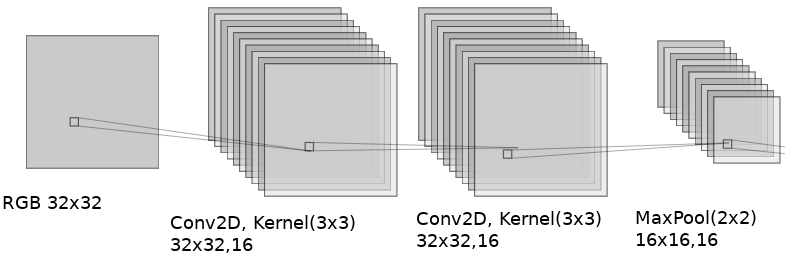
\includegraphics[scale=0.4]{pictures/Cifar_10_lite/cnn1}
\end{figure}
\end{frame}

\begin{frame}[fragile]
\frametitle{CNN for Cifar-10 classification on ST Cloud JAM}
\framesubtitle{Neural Network architecture}
\begin{figure}
	\centering
	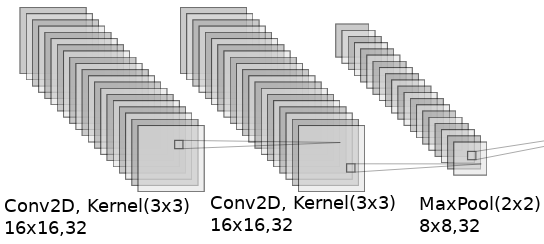
\includegraphics[scale=0.4]{pictures/Cifar_10_lite/cnn2}
\end{figure}
\end{frame}

\begin{frame}[fragile]
\frametitle{CNN for Cifar-10 classification on ST Cloud JAM}
\framesubtitle{Neural Network architecture}
\begin{figure}
	\centering
	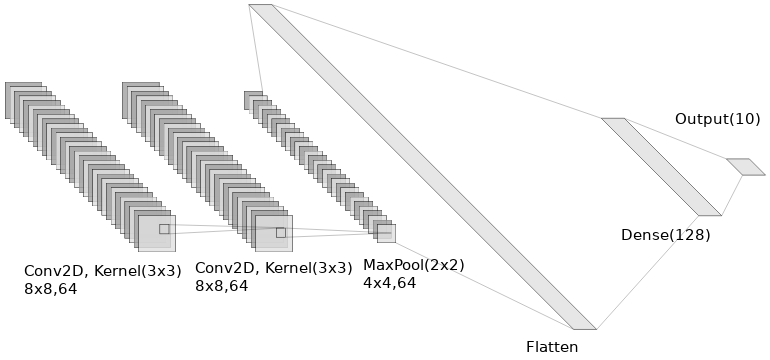
\includegraphics[scale=0.4]{pictures/Cifar_10_lite/cnn3}
\end{figure}
\end{frame}

\begin{frame}[fragile]
\frametitle{CNN for Cifar-10 classification on ST Cloud JAM}
\framesubtitle{Accuracy}
\begin{figure}[ht]
	\centering
	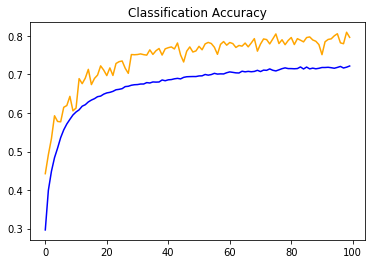
\includegraphics[scale=0.5]{pictures/Accuracy_plot_Cifar10_Keras_Lite}
	\begin{lstlisting}
	Epoch 100/100
	782/782 [==============================] - 43s 55ms/step - loss: 0.8155 - acc: 0.7220 - val_loss: 0.5932 - val_acc: 0.7963
	\end{lstlisting}
\end{figure}
\end{frame}

\begin{frame}[fragile]
\frametitle{Test CNN con Cifar-10 su ST Cloud JAM}
\framesubtitle{Validation on target of the Neural Network}
\small{The network is imported without weights compression. The L2R error betwen the results on host (computer) and target is in the order of \(10^-6\)}
\lstset{basicstyle=\ttfamily\scriptsize\color{black},backgroundcolor=\color{backcolour},keywordstyle=\color{black},commentstyle=\color{black}}
\begin{lstlisting}
acc=100.00%, rmse=0.0000, mae=0.0000
10 classes (1000 samples)
----------------------------------------------------------
C0         0    .    .    .    .    .    .    .    .    .  
C1         .   508   .    .    .    .    .    .    .    .  
C2         .    .    0    .    .    .    .    .    .    .  
C3         .    .    .    0    .    .    .    .    .    .  
C4         .    .    .    .    0    .    .    .    .    .  
C5         .    .    .    .    .   14    .    .    .    .  
C6         .    .    .    .    .    .    0    .    .    .  
C7         .    .    .    .    .    .    .    5    .    .  
C8         .    .    .    .    .    .    .    .    2    .  
C9         .    .    .    .    .    .    .    .    .   471 

Evaluation report (summary)
--------------------------------------------------
Mode                   acc       rmse      mae      
--------------------------------------------------
X-cross #1             100.0%    0.000001  0.000000 
L2r error : 4.15037266e-06 (expected to be < 0.01)
\end{lstlisting}
\end{frame}

\begin{frame}
\frametitle{CNN for Cifar-100 classification on computer}
\framesubtitle{Neural Network architecture}
\begin{figure}
	\centering
	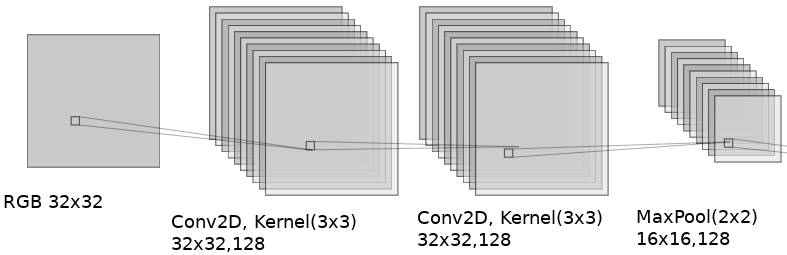
\includegraphics[scale=0.4]{pictures/Cifar_100/cnn1}
\end{figure}
\end{frame}

\begin{frame}
\frametitle{CNN for Cifar-100 classification on computer}
\framesubtitle{Neural Network architecture}
\begin{figure}
	\centering
	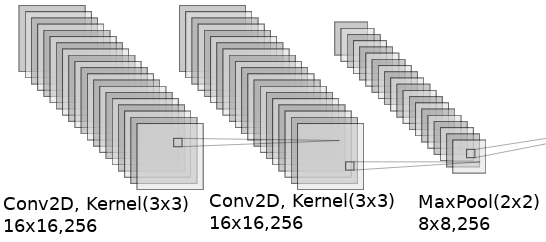
\includegraphics[scale=0.4]{pictures/Cifar_100/cnn2}
\end{figure}
\end{frame}

\begin{frame}
\frametitle{CNN for Cifar-100 classification on computer}
\framesubtitle{Neural Network architecture}
\begin{figure}
	\centering
	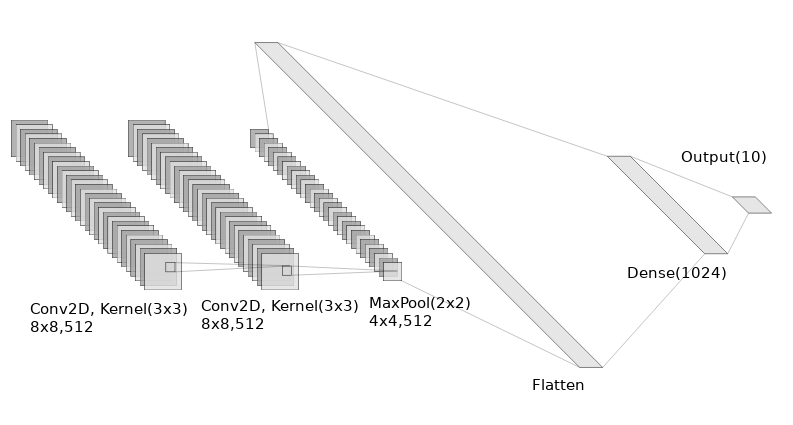
\includegraphics[scale=0.4]{pictures/Cifar_100/cnn3}
\end{figure}
\end{frame}

\begin{frame}[fragile]
\frametitle{Cifar-100 random images}
\begin{figure}
	\centering
	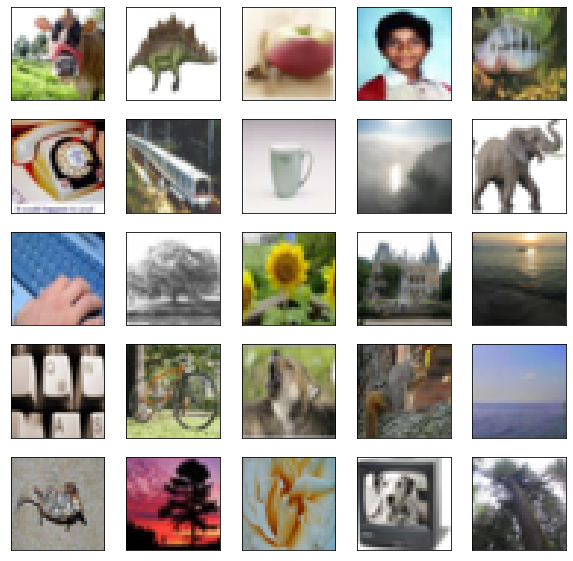
\includegraphics[scale=0.35]{pictures/index_Cifar-100}
\end{figure}
\end{frame}

\begin{frame}[fragile]
\frametitle{CNN for Cifar-100 classification on computer}
\framesubtitle{Accuracy}
\centering
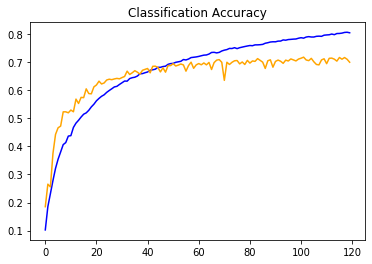
\includegraphics[scale=0.5]{pictures/Accuracy_plot_Cifar100_Keras}
\begin{lstlisting}
Epoch 120/120
782/782 [==============================] - 50s 64ms/step - loss: 0.6304 - acc: 0.8049 - val_loss: 1.2676 - val_acc: 0.7001
\end{lstlisting}
\end{frame}

\begin{frame}[fragile]
\frametitle{Test CNN con Cifar-100 su ST Cloud JAM}
\framesubtitle{Validation on target of the Neural Network}
\small{The network is imported without weights compression. The L2R error betwen the results on host (computer) and target is in the order of \(10^-6\)}
\lstset{basicstyle=\ttfamily\footnotesize\color{black},backgroundcolor=\color{backcolour},keywordstyle=\color{black},commentstyle=\color{black}}
\begin{lstlisting}
Running with inputs (1000, 32, 32, 3)..
\end{lstlisting}

\begin{lstlisting}
acc=100.00%, rmse=0.0000, mae=0.0000



Evaluation report (summary)
--------------------------------------------------
Mode                   acc       rmse      mae      
--------------------------------------------------
X-cross #1             100.0%    0.000000  0.000000 

L2r error : 1.32934053e-06 (expected to be < 0.01)
\end{lstlisting}
\end{frame}

\begin{frame}
\frametitle{CNN for Cifar-100 classification on Coral Edge TPU}
\framesubtitle{Introduction}
Coral USB Accelerator is a device aimed to support a calculator with an operating system.
\begin{figure}
	\centering
	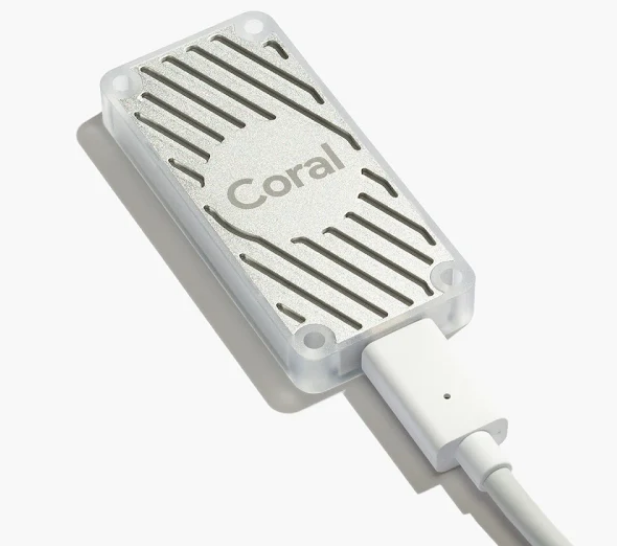
\includegraphics[scale=0.3]{pictures/coral_photo}
\end{figure}
\end{frame}

\begin{frame}[fragile]
\frametitle{CNN for Cifar-100 classification on Coral Edge TPU}
\framesubtitle{Requirement, Structure}
	\begin{figure}
		\centering
		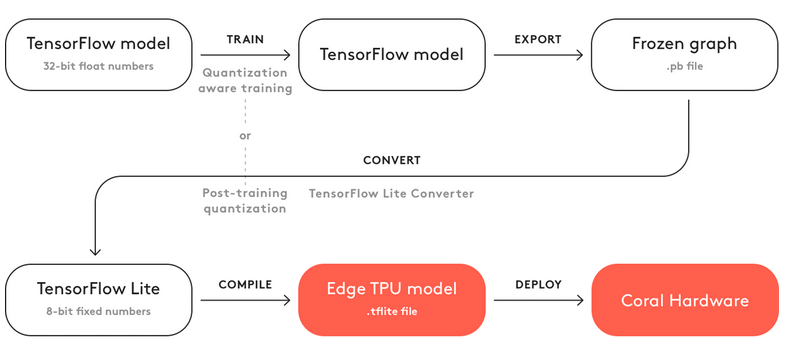
\includegraphics[scale=0.4]{pictures/passi_coral}
	\end{figure}
\end{frame}

\begin{frame}[fragile]
\frametitle{CNN for Cifar-100 classification on Coral Edge TPU}
\framesubtitle{Requirement, Structure}
\begin{lstlisting}
def cnn_model_fn(features, labels, mode):
    with tf.name_scope('model_input') as scope:
    input_layer = tf.reshape(features, [-1, 32, 32, 3], name="input")
    
    with tf.name_scope('model_conv1') as scope:
    conv1 = tf.layers.conv2d(inputs=input_layer, filters=32, kernel_size=[2, 2],
    padding="same", activation=tf.nn.relu6,
    trainable=mode == tf.estimator.ModeKeys.TRAIN)
    
    with tf.name_scope('model_conv2') as scope:
    conv2 = tf.layers.conv2d(inputs=conv1, filters=32, kernel_size=[2, 2],
    padding="same", activation=tf.nn.relu6,
    trainable=mode == tf.estimator.ModeKeys.TRAIN)
    
    pool1 = tf.layers.max_pooling2d(inputs=conv2, pool_size=[2, 2], strides=(2, 2))
    drop1 = tf.layers.dropout(inputs=pool1, rate=0.2)
\end{lstlisting}
\end{frame}

\begin{frame}[fragile]
\frametitle{CNN for Cifar-100 classification on Coral Edge TPU}
\framesubtitle{Requirement, Structure}
\begin{lstlisting}
    with tf.name_scope('model_conv3') as scope:
    conv3 = tf.layers.conv2d(inputs=drop1, filters=64, kernel_size=[2, 2],
    padding="same", activation=tf.nn.relu6,
    trainable=mode == tf.estimator.ModeKeys.TRAIN)
    
    with tf.name_scope('model_conv4') as scope:
    conv4 = tf.layers.conv2d(inputs=conv3, filters=64, kernel_size=[2, 2],
    padding="same", activation=tf.nn.relu6,
    trainable=mode == tf.estimator.ModeKeys.TRAIN)
    pool2 = tf.layers.max_pooling2d(inputs=conv4, pool_size=[2, 2], strides=(2, 2))
    drop2 = tf.layers.dropout(inputs=pool2, rate=0.3)
\end{lstlisting}
\end{frame}

\begin{frame}[fragile]
\frametitle{CNN for Cifar-100 classification on Coral Edge TPU}
\framesubtitle{Tensorflow network definition}
\begin{lstlisting}
    with tf.name_scope('model_conv5') as scope:
    conv5 = tf.layers.conv2d(inputs=drop2, filters=128, kernel_size=[2, 2],
    padding="same", activation=tf.nn.relu6,
    trainable=mode == tf.estimator.ModeKeys.TRAIN)
    
    with tf.name_scope('model_conv6') as scope:
    conv6 = tf.layers.conv2d(inputs=conv5, filters=128, kernel_size=[2, 2],
    padding="same", activation=tf.nn.relu6,
    trainable=mode == tf.estimator.ModeKeys.TRAIN)
    pool3 = tf.layers.max_pooling2d(inputs=conv6, pool_size=[2, 2], strides=(2, 2))
    drop3 = tf.layers.dropout(inputs=pool3, rate=0.4)
\end{lstlisting}
\end{frame}

\begin{frame}[fragile]
\frametitle{CNN for Cifar-100 classification on Coral Edge TPU}
\framesubtitle{Tensorflow network definition}
\begin{lstlisting}
    with tf.name_scope('model_dense') as scope:
    flat = tf.reshape(drop3, [-1, 4 * 4 * 128])
    
    dense = tf.layers.dense(inputs=flat, units=1024,
    activation=tf.nn.relu6,
    trainable=mode == tf.estimator.ModeKeys.TRAIN)
    
    drop4 = tf.layers.dropout(inputs=dense, rate=0.5, training=mode == tf.estimator.ModeKeys.TRAIN)
    
    with tf.name_scope('model_output') as scope:
    logits = tf.layers.dense(inputs=drop4, units=10, trainable=mode == tf.estimator.ModeKeys.TRAIN)
    
    predictions = {latin1
    "classes": tf.argmax(inputlatin1=logits, axis=1),
    "probabilities": tf.nn.soflatin1tmax(logits, name="softmax_tensor")
}
\end{lstlisting}
\end{frame}

\begin{frame}[fragile]
\frametitle{CNN for Cifar-100 classification on Coral Edge TPU}
\framesubtitle{Tensorflow network definition}
\begin{lstlisting}
    # TRAIN mode
    if mode == tf.estimator.ModeKeys.TRAIN:
    g = tf.get_default_graph()
    tf.contrib.quantize.create_training_graph(input_graph=g, quant_delay=6000)
    optimizer = tf.train.AdamOptimizer(learning_rate=0.001)
    train_op = optimizer.minimize(
    loss=loss,
    global_step=tf.train.get_global_step())
    return tf.estimator.EstimatorSpec(mode=mode, loss=loss, train_op=train_op)
    
    # EVAL mode
    g = tf.get_default_graph()
    tf.contrib.quantize.create_eval_graph(input_graph=g)
    labels = tf.argmax(labels, axis=1)
    eval_metric_ops = {
    "accuracy": tf.metrics.accuracy(labels=labels, predictions=predictions["classes"])
}
return tf.estimator.EstimatorSpec(
mode=mode, loss=loss, eval_metric_ops=eval_metric_ops)
\end{lstlisting}
\end{frame}


\begin{frame}[fragile]
\frametitle{CNN for Cifar-100 classification on Coral Edge TPU}
\framesubtitle{Training and saving}
\textbf{Training:}
\begin{lstlisting}
def fit_all_batches(xEpochs):
    # Train the model
    train_input_fn = tf.estimator.inputs.numpy_input_fn(
    x=train_features,
    y=train_labels,
    batch_size=32,
    num_epochs=xEpochs,
    shuffle=False)
    
    # train one step and display the probabilties
    cifar10_classifier.train(
    input_fn=train_input_fn,
    steps=None,
    hooks=[logging_hook])
	
fit_all_batches(100)
\end{lstlisting}
\textbf{Saving in .pb format:}
\begin{lstlisting}
cifar10_classifier.experimental_export_all_saved_models(
savedir,
input_receiver_fn_map)
\end{lstlisting}
\end{frame}

\begin{frame}[fragile]
\frametitle{CNN for Cifar-100 classification on Coral Edge TPU}
\framesubtitle{Accuracy and test}
\lstset{basicstyle=\ttfamily\scriptsize\color{black},backgroundcolor=\color{backcolour},keywordstyle=\color{black},stringstyle=\color{black}}
\begin{lstlisting}
{'accuracy': 0.7656, 'loss': 1.5887853, 'global_step': 142032}
\end{lstlisting}
\begin{lstlisting}
[['airplane' '0.9999999']
['automobile' '1.5820127e-23']
['bird' '6.063283e-08']
['cat' '7.3694817e-10']
['deer' '2.7018123e-08']
['dog' '1.1388865e-14']
['frog' '5.9821274e-15']
['horse' '1.180477e-18']
['ship' '8.983325e-14']
['truck' '2.4614857e-21']]
\end{lstlisting}
\vspace{-2mm}
\begin{figure}
	\centering
	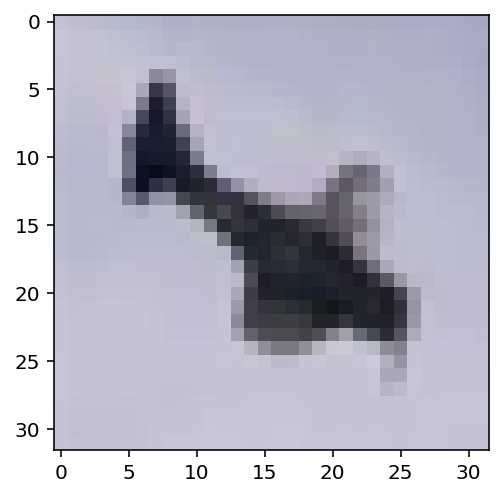
\includegraphics[scale=0.4]{pictures/Classifica_immagine_casuale_Tensorflow1}
\end{figure}
\end{frame}

\begin{frame}[fragile]
\frametitle{CNN for Cifar-100 classification on Coral Edge TPU}
\framesubtitle{Frozen graph creation}
script Python \verb+freeze_graph.py+\\
\begin{lstlisting}
tf.saved_model.loader.load(sess,["serve"],savedir )

from tensorflow.python.tools import freeze_graph
from tensorflow.python.saved_model import tag_constants

input_graph_filename = None
input_saved_model_dir = savedir
output_node_names = "softmax_tensor"
output_graph_filename = os.path.join(savedir,"frozen.pb")
input_binary = False
input_saver_def_path = False
restore_op_name = None
filename_tensor_name = None
clear_devices = True
input_meta_graph = False
checkpoint_path = None
\end{lstlisting}
\end{frame}

\begin{frame}[fragile]
\frametitle{CNN for Cifar-100 classification on Coral Edge TPU}
\framesubtitle{TFlite conversion}
\textbf{TOCO} converter, disponibile con Tensorflow
\lstset{basicstyle=\ttfamily\footnotesize\color{white},backgroundcolor=\color{backgroundblack},keywordstyle=\color{white}
numberstyle=\color{white},stringstyle=\color{white}}
\begin{lstlisting}
toco \
--input_file=frozen.pb \
--output_file=tflite_model.tflite \
--input_format=TENSORFLOW_GRAPHDEF \
--output_format=TFLITE \
--inference_type=QUANTIZED_UINT8 \
--input_shape="1,32,32,3" \
--input_array=model_input/input \
--output_array=softmax_tensor \
--std_dev_values=127 \
--mean_value=127 \
--default_ranges_min=0 \
--default_ranges_max=6
\end{lstlisting}
\end{frame}


\begin{frame}[fragile]
\frametitle{CNN for Cifar-100 classification on Coral Edge TPU}
\framesubtitle{Compilation}
\textbf{Edge TPU Compiler}\\
\(\rightarrow\) conversione da TF Lite a in un modello per Coral USB Accelerator
\lstset{basicstyle=\ttfamily\footnotesize\color{white},backgroundcolor=\color{backgroundblack},keywordstyle=\color{white}
	numberstyle=\color{white},stringstyle=\color{white}}
\begin{lstlisting}
edgetpu_compiler [options] model...
\end{lstlisting}
\end{frame}

\begin{frame}[fragile]
\frametitle{CNN for Cifar-100 classification on Coral Edge TPU}
\framesubtitle{Classification}
\textbf{Classificatore:} \verb+CIFAR10_Inference_EdgeTPU.py+
\lstset{basicstyle=\ttfamily\footnotesize\color{white},backgroundcolor=\color{backgroundblack},keywordstyle=\color{white}
	numberstyle=\color{white},stringstyle=\color{white},keywordstyle=\color{white}}
\begin{lstlisting}
python3 my_classifier.py --model=/home/matteo/Documents/Frozen/Compiled_models/frozen_edgetpu.tflite --image=/home/matteo/Downloads/cifar10_images/truck3.png 
WARNING:root:From my_classifier.py:30: The name ClassifyWithImage will be deprecated. Please use classify_with_image instead.

---------------------------
truck
Score :  0.99609375
Elapsed time for the last inference:  0.03292989730834961
\end{lstlisting}
\end{frame}

\begin{frame}[fragile]
\frametitle{CNN for Cifar-100 classification on Coral Edge TPU}
\framesubtitle{Classification}
\lstset{basicstyle=\ttfamily\footnotesize\color{white},backgroundcolor=\color{backgroundblack},keywordstyle=\color{white}
	numberstyle=\color{white},stringstyle=\color{white},keywordstyle=\color{white}}
\begin{lstlisting}
python3 my_classifier.py --model=/home/matteo/Documents/Frozen/Compiled_models/frozen_example_min_max_edgetpu.tflite --image=/home/matteo/Downloads/cifar10_images/bird3.png 
WARNING:root:From my_classifier.py:30: The name ClassifyWithImage will be deprecated. Please use classify_with_image instead.

---------------------------
truck
Score :  0.62890625
---------------------------
frog
Score :  0.2890625
Elapsed time for the last inference:  0.03208661079406738
\end{lstlisting}
\end{frame}



\end{document}


